\documentclass[12pt]{article}
\usepackage{pslatex}
\usepackage{apacite}
\usepackage{amsmath}  % math symbols
\usepackage{amssymb}
\usepackage{amsthm}
\usepackage[scale={0.8,0.9}, centering, includeheadfoot]{geometry}
\usepackage{tikz}
\usetikzlibrary{decorations.pathreplacing,positioning, fit, arrows.meta, shapes}
\usetikzlibrary{shapes}
\usepackage{float}
\usepackage{natbib}
\usepackage{subcaption}
\usepackage{caption}
\usepackage{booktabs}
\usepackage{xcolor}
\usepackage{colortbl}
\usepackage{multirow}

\usepackage[]{titlesec}
\titlespacing*{\section}{0pt}{1.6ex}{.5ex}
\titlespacing*{\subsection}{0pt}{1ex}{.5ex}
\titlespacing*{\subsubsection}{0pt}{.5ex}{.5ex}
\titleformat{\section}{\large\bfseries}{\thesection}{1em}{}
\titleformat{\subsection}{\normalsize\bfseries}{\thesubsection}{1em}{}

\newcommand{\inputcolor}{black!20}
\newcommand{\outputcolor}{red!40}
\newcommand{\hiddencolor}{blue!40}
\newcommand{\hiddencolortwo}{orange!40}
\newcommand{\colorlabel}{green!40}
\newcommand{\compare}{cosine}

\newcommand{\softmax}{\mathbf{softmax}}
\DeclareMathOperator{\ReLU}{ReLU}
\newcommand{\identity}{\mathbb{I}}
\newcommand{\LSTM}{\textbf{LSTM}}

% Flexible sec/fig/tbl/def cross-refs.
\newcommand{\Secref}[1]{Sec.~\ref{#1}}
\newcommand{\secref}[1]{sec.~\ref{#1}}
\newcommand{\dashsecref}[2]{secs.~\ref{#1}--\ref{#2}}

\newcommand{\Figref}[1]{Fig.~\ref{#1}}
\newcommand{\figref}[1]{fig.~\ref{#1}}
\newcommand{\dashfigref}[2]{figs.~\ref{#1}--\ref{#2}}
\newcommand{\Tabref}[1]{Tab.~\ref{#1}}
\newcommand{\tabref}[1]{tab.~\ref{#1}}

% Examples:
\newcommand{\eg}[1]{(\ref{#1})}
\newcommand{\dasheg}[2]{\eg{#1}--\eg{#2}}
\newcommand{\subeg}[2]{(\ref{#1}\ref{#2})}
\newcommand{\dblsubeg}[3]{(\ref{#1}\ref{#2},~\ref{#3})}
\newcommand{\dashsubeg}[3]{(\ref{#1}\ref{#2}--\ref{#3})}

%=====================================================================
%=====================================================================

\title{Supplementary materials for `Relational reasoning and generalization using non-symbolic neural networks'}
\author{Anonymous CogSci 2020 submission}
\date{}

%=====================================================================
%=====================================================================

\begin{document}
\maketitle

\tableofcontents

\newpage


%=====================================================================
%=====================================================================

\section{Model figures}


%=====================================================================

\subsection{Model 1: Same--different relation with feed-foward  networks}\label{sec:model1}

Our model of equality is given by \dasheg{eq:x2h}{eq:h2y}:
%
\begin{align}
  h &= \ReLU([a;b]W_{xh} + b_{h}) \label{eq:x2h}\\
  y &= \softmax(hW_{hy} + b_{y}) \label{eq:h2y}
\end{align}
%
where $a$ and $b$ have dimension $m$ (the embedding dimension), $W_{xh}$ is a weight matrix of dimension $2m \times n$, $b_{h}$ is a bias vector of dimension $n$, $W_{hy}$ is a weight matrix of dimension $n \times 2$, $b_{y}$ is a bias vector of dimension $2$, $\ReLU(x) = \max(0, x)$, and $\softmax(x)_{i} = \frac{\exp{x_{i}}}{\sum_{j} \exp{x_{j}}}$.

\Figref{fig:models:equality} provides a visual depiction of the model. The gray boxes correspond to embedding representations, the purple box is the hidden representation $h$, and the red box is the output distribution $y$. Dotted arrows depict concatenation, and solid arrows depict the dense relations corresponding to the matrix multiplications (plus bias terms) in \dasheg{eq:x2h}{eq:h2y}.

\begin{figure}[H]
  \centering
  \resizebox{100pt}{!}{%
    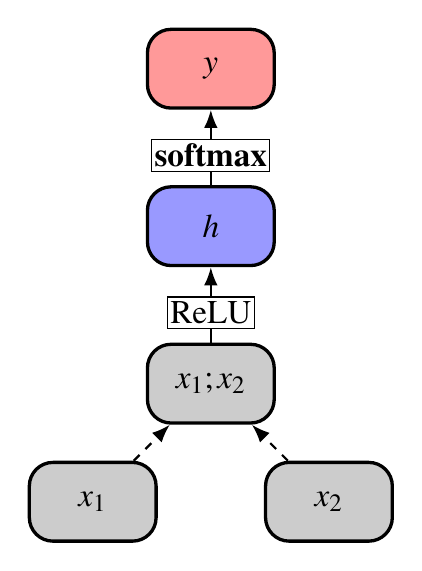
\begin{tikzpicture}[
      % GLOBAL CFG
      font=\sf \large,
      >=LaTeX,
      % Styles
      rep/.style={% For representations
        rectangle,
        rounded corners=3mm,
        draw,
        very thick,
        minimum height =1cm,
        minimum width=1.61cm
      },
      function/.style={%For functions
        ellipse,
        draw,
        inner sep=1pt
      },
      gt/.style={% For internal inputs
        rectangle,
        draw,
        minimum width=5mm,
        minimum height=4mm,
        inner sep=1pt
      },
      function/.style={
        rectangle,
        draw,
        minimum width=5mm,
        minimum height=4mm,
        inner sep=1pt
      },
      arrowconcat/.style={% Arrows for concatenation
        rounded corners=.25cm,
        dashed,
        thick,
        ->,
      },
      arrowfunction/.style={% Arrows for concatenation
        rounded corners=.25cm,
        thick,
        ->,
      }
      ]

      % Start drawing the thing...
      % Draw the cell:
      \node [rep, fill=\inputcolor] (input1) at (-1.5,1.5){$x_1$} ;
      \node [rep, fill=\inputcolor] (input2) at (1.5,1.5){$x_2$} ;
      \node [rep, fill=\inputcolor] (concat) at (0,3){$x_1;x_2$} ;
      \draw [arrowconcat] (input1) -- (concat);
      \draw [arrowconcat] (input2) -- (concat);


      \node [rep, fill=\hiddencolor] (hidden) at (0,5){$h$} ;
      \node [gt, minimum width=1cm] (relu) at (0,4-0.1) {$\ReLU$};
      \draw [arrowfunction] (concat) -- (relu) -- (hidden);


      \node [rep,fill=\outputcolor] (output) at (0,7){$y$} ;
      \node [gt, minimum width=1cm] (softmax) at (0,6-0.1) {$\softmax$};
      \draw [arrowfunction] (hidden) -- (softmax) -- (output);

    \end{tikzpicture}
  }
  \caption{A single layer network computing equality.}
  \label{fig:models:equality}
\end{figure}


%=====================================================================

\subsection{Model 2: Sequential same--different (ABA task)}\label{sec:model2}

The specific model we use for this is as follows:
%
\begin{align}
  h_{t} &= \LSTM(x_{t}, h_{t-1}) \label{eq:lstm-recur}\\
  y_{t} &= h_{t}W + b\label{eq:lstm-predict}
\end{align}
%
for $t > 0$, with $h_{0} = \mathbf{0}$. $\LSTM$ is a long short-term memory cell. \Figref{fig:reps:sequence} depicts this model. At each timestep $t$, a vector $y_{t}$ (red) is predicted based on the input representation at $t$ (gray) and the hidden representation at $t$ (purple). During training, this is compared with the actual vector for timestep $t+1$ (green). During testing, the predicted vector $y_{i}$ is compared with every item in the union of the train and assessment vocabularies, and the closest vector (according to cosine similarity) is taken to be the prediction. This vector is then used as the input for timestep $t+1$.

\begin{figure}[H]
  \centering
  \resizebox{350pt}{!}{%
    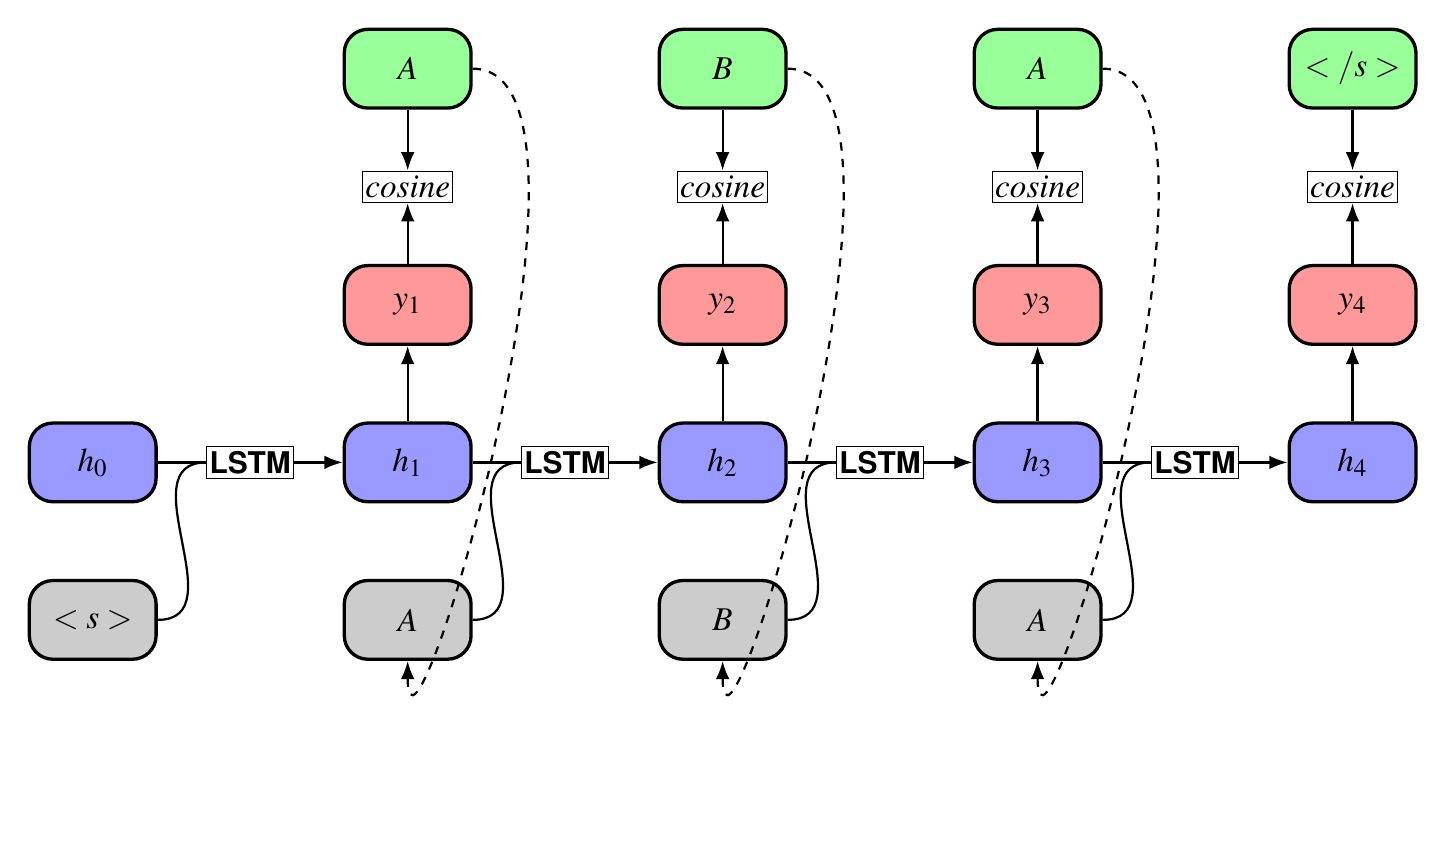
\begin{tikzpicture}[
      % GLOBAL CFG
      font=\sf \large,
      >=LaTeX,
      % Styles
      rep/.style={% For representations
        rectangle,
        rounded corners=3mm,
        draw,
        very thick,
        minimum height =1cm,
        minimum width=1.61cm
      },
      function/.style={%For functions
        ellipse,
        draw,
        inner sep=1pt
      },
      gt/.style={% For internal inputs
        rectangle,
        draw,
        minimum width=5mm,
        minimum height=4mm,
        inner sep=1pt
      },
      function/.style={
        rectangle,
        draw,
        minimum width=5mm,
        minimum height=4mm,
        inner sep=1pt
      },
      arrowconcat/.style={% Arrows for concatenation
        rounded corners=.25cm,
        dashed,
        thick,
        ->,
      },
      arrowfunction/.style={% Arrows for concatenation
        rounded corners=.25cm,
        thick,
        ->,
      }
      ]

      % Start drawing the thing...
      % Draw the cell:
      \node [rep, fill=\inputcolor] (input1) at (-10,4){$<s>$} ;
      \node [rep, fill=\inputcolor] (input2) at (-6,4){$A$} ;
      \node [rep, fill=\inputcolor] (input3) at (-2,4){$B$} ;
      \node [rep, fill=\inputcolor] (input4) at (2,4){$A$} ;

      \node [rep, fill=\hiddencolor] (hidden0) at (-10,6){$h_0$} ;
      \node [rep, fill=\hiddencolor] (hidden1) at (-6,6){$h_1$} ;
      \node [rep, fill=\hiddencolor] (hidden2) at (-2,6){$h_2$} ;
      \node [rep, fill=\hiddencolor] (hidden3) at (2,6){$h_3$} ;
      \node [rep, fill=\hiddencolor] (hidden4) at (6,6){$h_4$} ;

      \node [gt] (LSTM0) at (-8,6){$\LSTM$} ;
      \node [gt] (LSTM1) at (-4,6){$\LSTM$} ;
      \node [gt] (LSTM2) at (0,6){$\LSTM$} ;
      \node [gt] (LSTM3) at (4,6){$\LSTM$} ;

      \node [rep, fill=\outputcolor] (output1) at (-6,8){$y_1$} ;
      \node [rep, fill=\outputcolor] (output2) at (-2,8){$y_2$} ;
      \node [rep, fill=\outputcolor] (output3) at (2,8){$y_3$} ;
      \node [rep, fill=\outputcolor] (output4) at (6,8){$y_4$} ;

      \node [gt] (compare1) at (-6,9.5){$\compare$} ;
      \node [gt] (compare2) at (-2,9.5){$\compare$} ;
      \node [gt] (compare3) at (2,9.5){$\compare$} ;
      \node [gt] (compare4) at (6,9.5){$\compare$} ;

      \node [rep, fill=\colorlabel] (label1) at (-6,11){$A$} ;
      \node [rep, fill=\colorlabel] (label2) at (-2,11){$B$} ;
      \node [rep, fill=\colorlabel] (label3) at (2,11){$A$} ;
      \node [rep, fill=\colorlabel] (label4) at (6,11){$</s>$} ;

      \draw [arrowfunction] (label1) -- (compare1);
      \draw [arrowfunction] (label2) -- (compare2);
      \draw [arrowfunction] (label3) -- (compare3);
      \draw [arrowfunction] (label4) -- (compare4);

      \draw [arrowfunction] (output1) -- (compare1);
      \draw [arrowfunction] (output2) -- (compare2);
      \draw [arrowfunction] (output3) -- (compare3);
      \draw [arrowfunction] (output4) -- (compare4);

      \draw [arrowfunction] (hidden1) -- (output1);
      \draw [arrowfunction] (hidden2) -- (output2);
      \draw [arrowfunction] (hidden3) -- (output3);
      \draw [arrowfunction] (hidden4) -- (output4);

      \draw [thick] (input1) to[out=0,in=-180, distance=1cm] (LSTM0);
      \draw [thick] (input2) to[out=0,in=-180, distance=1cm] (LSTM1);
      \draw [thick] (input3) to[out=0,in=-180, distance=1cm] (LSTM2);
      \draw [thick] (input4) to[out=0,in=-180, distance=1cm] (LSTM3);

      \draw [arrowfunction] (hidden0) -- (LSTM0) -- (hidden1);
      \draw [arrowfunction] (hidden1) -- (LSTM1)-- (hidden2);
      \draw [arrowfunction] (hidden2) -- (LSTM2)-- (hidden3);
      \draw [arrowfunction] (hidden3) -- (LSTM3)-- (hidden4);

      \draw[->,dashed,thick] (label1) to[out=0,in=-90, distance=1.99cm] (input2);
      \draw[->,dashed,thick] (label2) to[out=0,in=-90, distance=1.99cm] (input3);
      \draw[->,dashed,thick] (label3) to[out=0,in=-90, distance=1.99cm] (input4);
    \end{tikzpicture}
  }
  \caption{A recursive LSTM network producing ABA sequences.}
  \label{fig:reps:sequence}
\end{figure}


%=====================================================================

\subsection{Model 3a: A deeper feed-forward network for hierarchical same--different}\label{sec:model3a}

This model extends \dasheg{eq:x2h}{eq:h2y} with an additional hidden layer and a larger input dimensionality, corresponding to the input pair of pairs $((a,b) (c,d))$ being flattened into a single concatenated representation $[a;b;c;d]$.
%
\begin{align}
  h_{1} &= \ReLU([a;b;c;d]W_{xh} + b_{h_{1}}) \label{eq:x2h1}\\
  h_{2} &= \ReLU(h_{1}W_{hh} + b_{h_{2}}) \label{eq:x2h2}\\
  y &= \softmax(h_{2}W_{hy} + b_{y}) \label{eq:h2y2}
\end{align}
%
\Figref{fig:models:premack-deep} depicts this model.

\begin{figure}[H]
  \centering
  \resizebox{150pt}{!}{%
    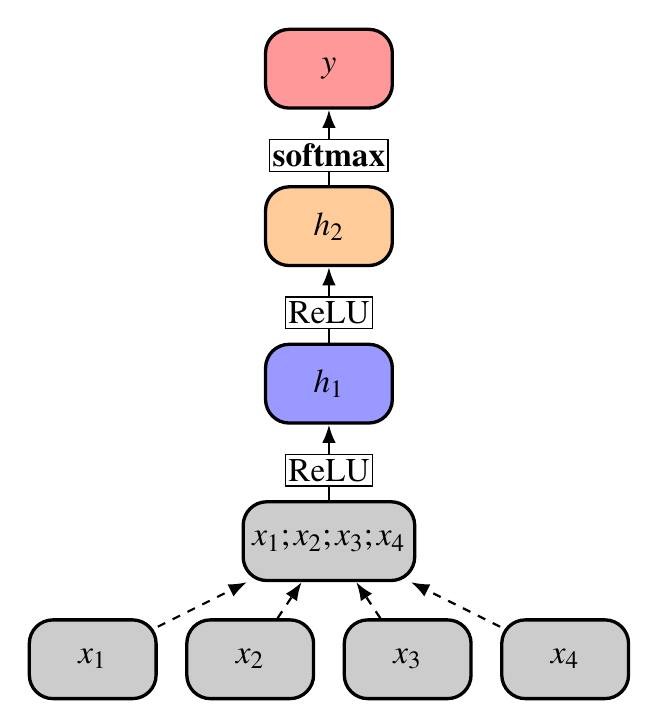
\begin{tikzpicture}[
      % GLOBAL CFG
      font=\sf \large,
      >=LaTeX,
      % Styles
      rep/.style={% For representations
        rectangle,
        rounded corners=3mm,
        draw,
        very thick,
        minimum height =1cm,
        minimum width=1.61cm
      },
      function/.style={%For functions
        ellipse,
        draw,
        inner sep=1pt
      },
      gt/.style={% For internal inputs
        rectangle,
        draw,
        minimum width=5mm,
        minimum height=4mm,
        inner sep=1pt
      },
      function/.style={
        rectangle,
        draw,
        minimum width=5mm,
        minimum height=4mm,
        inner sep=1pt
      },
      arrowconcat/.style={% Arrows for concatenation
        rounded corners=.25cm,
        dashed,
        thick,
        ->,
      },
      arrowfunction/.style={% Arrows for concatenation
        rounded corners=.25cm,
        thick,
        ->,
      }
      ]

      % Start drawing the thing...
      % Draw the cell:
      \node [rep, fill=\inputcolor] (input1) at (-3,1.5){$x_1$} ;
      \node [rep, fill=\inputcolor] (input2) at (-1,1.5){$x_2$} ;
      \node [rep, fill=\inputcolor] (input3) at (1,1.5){$x_3$} ;
      \node [rep, fill=\inputcolor] (input4) at (3,1.5){$x_4$} ;
      \node [rep, fill=\inputcolor] (concat) at (0,3){$x_1;x_2;x_3;x_4$} ;
      \draw [arrowconcat] (input1) -- (concat);
      \draw [arrowconcat] (input2) -- (concat);
      \draw [arrowconcat] (input3) -- (concat);
      \draw [arrowconcat] (input4) -- (concat);


      \node [rep, fill=\hiddencolor] (hidden) at (0,5){$h_1$} ;
      \node [gt, minimum width=1cm] (relu) at (0,4-0.1) {$\ReLU$};
      \draw [arrowfunction] (concat) -- (relu) -- (hidden);

      \node [rep, fill=\hiddencolortwo] (hidden2) at (0,7){$h_2$} ;
      \node [gt, minimum width=1cm] (relu2) at (0,6-0.1) {$\ReLU$};
      \draw [arrowfunction] (hidden) -- (relu2) -- (hidden2);


      \node [rep,fill=\outputcolor] (output) at (0,9){$y$} ;
      \node [gt, minimum width=1cm] (softmax) at (0,8-0.1) {$\softmax$};
      \draw [arrowfunction] (hidden2) -- (softmax) -- (output);

    \end{tikzpicture}
  }
  \caption{A two layer network computing hierarchical equality.}
  \label{fig:models:premack-deep}
\end{figure}


%=====================================================================

\subsection{Model 3b: Pretraining for hierarchical same--different}\label{sec:model3b}

Our pretraining model is as follows:
%
\begin{align}
  h_1 &= \ReLU([a;b]W_{xh} + b_{h}) \label{eq:preh1}\\
  h_2 &= \ReLU([c;d]W_{xh} + b_{h})\\
  h_3 &= \ReLU([h_1;h_2]W_{xh} + b_{h}) \\
  y &= \softmax(h_3W_{hy} + b_{y}) \label{eq:prey}\
\end{align}
%
where $W_{xh}$, $W_{hy}$, $b_h$, and $b_y$ are the parameters from the model in \dasheg{eq:x2h}{eq:h2y} already trained on basic equality. \Figref{fig:models:premack} depicts this model. The colors indicate where parameters are reused by the model.


\begin{figure}[H]
  \centering
  \resizebox{250pt}{!}{%
    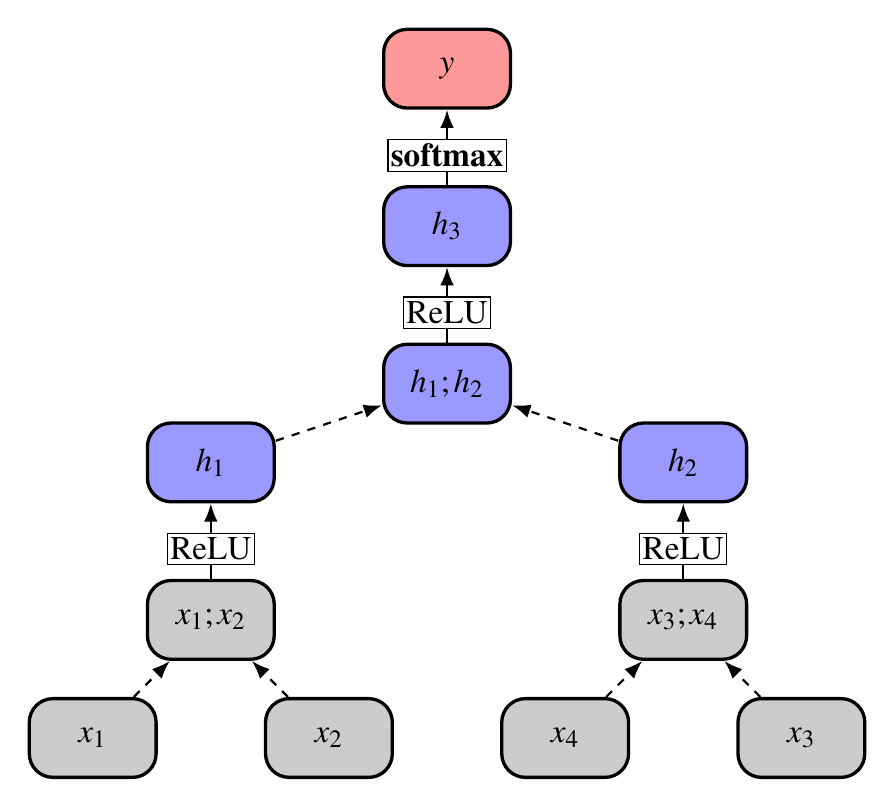
\begin{tikzpicture}[
      % GLOBAL CFG
      font=\sf \large,
      >=LaTeX,
      % Styles
      rep/.style={% For representations
        rectangle,
        rounded corners=3mm,
        draw,
        very thick,
        minimum height =1cm,
        minimum width=1.61cm
      },
      function/.style={%For functions
        ellipse,
        draw,
        inner sep=1pt
      },
      gt/.style={% For internal inputs
        rectangle,
        draw,
        minimum width=5mm,
        minimum height=4mm,
        inner sep=1pt
      },
      function/.style={
        rectangle,
        draw,
        minimum width=5mm,
        minimum height=4mm,
        inner sep=1pt
      },
      arrowconcat/.style={% Arrows for concatenation
        rounded corners=.25cm,
        dashed,
        thick,
        ->,
      },
      arrowfunction/.style={% Arrows for concatenation
        rounded corners=.25cm,
        thick,
        ->,
      }
      ]

      % Start drawing the thing...
      % Draw the cell:
      \node [rep, fill=\inputcolor] (input1) at (-4.5,1.5){$x_1$} ;
      \node [rep, fill=\inputcolor] (input2) at (-1.5,1.5){$x_2$} ;
      \node [rep, fill=\inputcolor] (concat) at (-3,3){$x_1;x_2$} ;
      \draw [arrowconcat] (input1) -- (concat);
      \draw [arrowconcat] (input2) -- (concat);


      \node [rep, fill=\hiddencolor] (hidden) at (-3,5){$h_1$} ;
      \node [gt, minimum width=1cm] (relu1) at (-3,4-0.1) {$\ReLU$};
      \draw [arrowfunction] (concat) -- (relu1) -- (hidden);


      \node [rep, fill=\inputcolor] (input3) at (4.5,1.5){$x_3$} ;
      \node [rep, fill=\inputcolor] (input4) at (1.5,1.5){$x_4$} ;
      \node [rep, fill=\inputcolor] (concat2) at (3,3){$x_3;x_4$} ;
      \draw [arrowconcat] (input3) -- (concat2);
      \draw [arrowconcat] (input4) -- (concat2);


      \node [rep, fill=\hiddencolor] (hidden2) at (3,5){$h_2$} ;
      \node [gt, minimum width=1cm] (relu2) at (3,4-0.1) {$\ReLU$};
      \draw [arrowfunction] (concat2) -- (relu2) -- (hidden2);


      \node [rep,fill=\hiddencolor] (hiddenconcat) at (0,6){$h_1;h_2$};
      \draw [arrowconcat] (hidden2) -- (hiddenconcat);
      \draw [arrowconcat] (hidden) -- (hiddenconcat);


      \node [rep, fill=\hiddencolor] (hidden3) at (0,8){$h_3$} ;
      \node [gt, minimum width=1cm] (relu3) at (0,7-0.1) {$\ReLU$};
      \draw [arrowfunction] (hiddenconcat) -- (relu3) -- (hidden3);


      \node [rep,fill=\outputcolor] (output) at (0,10){$y$} ;
      \node [gt, minimum width=1cm] (softmax) at (0,9-0.1) {$\softmax$};
      \draw [arrowfunction] (hidden3) -- (softmax) -- (output);

    \end{tikzpicture}
  }
  \caption{A single layer network pretrained on equality computing hierarchical equality.}
  \label{fig:models:premack}
\end{figure}


%=====================================================================
%=====================================================================

\section{Model optimization details}

The feed forward networks for basic and hierarchical equality were implemented using the multi-layer perception from sklearn and a cross entropy function was used to compute the prediction error. The recursive LSTM network for the sequential ABA task was implemented using PyTorch and a mean squared error function was used to compute the prediction error. The network pretrained on basic equality and then used for hierarchical equality was implemented using TensorFlow and a cross entropy function was used to compute the prediction error. For all models, Adam optimizers were used. For all models, a hyperparameter search was run over learning rate values of \{0.00001, 0.0001, 0.001\} and l2 normalization values of \{0.0001, 0.001, 0.01\} for each hidden dimension and input dimension mentioned in the paper.


%=====================================================================
%=====================================================================

\section{Localist and binary feature representations prevent generalization}

The method of representation impacts whether there is a natural notion of similarity between entities and the ability of models to generalize to examples unseen in training. These two attributes are deeply related; if there is a natural notion of similarity between vector representations, then models can generalize to inputs with representations that are similar to those seen in training.

In order to discuss how representation impacts generalization, we will need explain some properties of how neural models are trained. Standard neural models, including all models in the paper, begin with applying a linear layer to the input vector where no two input units are connected to the same weight. A easily observed fact about the back-propagation learning algorithm is that if a unit of the input vector is always zero during training, then any weights connected to that unit and only that unit will not change from their initialized values during training. This means that when a standard neural model is evaluated on an input vector that has a non-zero value for a unit that was zero throughout training, untrained weights are used and behavior is unpredictable.

Localist representations are orthogonal and equidistant from one another so there is no notion of similarity and consequently standard neural models have no ability to generalize to new examples. No two representations share a non-zero unit, and so when models are presented with inputs unseen in training, untrained weights are used and behavior is unpredictable.

Distributed representations with binary features also limit generalization, though less severely than localist representations. Localist representations prevent generalization to entities unseen during training, while binary feature representations prevent generalization to features unseen during training. If color and shape are represented as binary features, and a red square and blue circle are seen in training, then a model could generalize to the unseen entities of a blue circle or a red square. However, if no entity that is a circle is seen during training, then the binary feature representing the property of being a circle is zero throughout training and untrained weights are used when the model is presented with a entity that is a circle during testing resulting in unpredictable behavior.

Distributed representations with analog features do not inhibit generalization in the same way. If height is represented as a binary feature, then a single unit represents all height values and is always non-zero. Random distributed representations similarly do not inhibit generalization, because all units for all representations are non-zero.


%=====================================================================
%=====================================================================

\section{An analytic solution to identity with a feed forward network}

Here are the parameters of a feed forward neural network that performs a binary classification task
%
\[ \texttt{ReLu}(\begin{pmatrix} x_1 \\ x_2  \end{pmatrix}^T \begin{pmatrix} W^{11} & W^{12}\\ W^{21}& W^{22} \end{pmatrix}) \begin{pmatrix} v^{11} & v^{12} \\ v^{21} & v^{22} \end{pmatrix} + \begin{pmatrix}b_1 &b_2 \end{pmatrix}= \begin{pmatrix} o_1 & o_2\end{pmatrix}\]
%
where if $n$ is the dimension of entity embeddings used then
\[
  x, y,v^{11}, v^{12}, v^{21}, v^{22} \in \mathbb{R}^{n \times 1}
\]
\[
  W^{11}, W^{12},W^{21}, W^{22} \in \mathbb{R}^{n \times n}
\]
\[
  b_1, b_2, o_1, o_2 \in \mathbb{R}
\]
Given an input $(x_1,x_2)$, if the output $o_1$ is larger than $o_2$ then one class is predicted and if the output $o_2$ is larger that $o_1$ then the other class is predicted. We when the two outputs are equal, the network has predicted that both classes are equally likely and we can arbitrarily decide which class is predicted. In this case, the output $o_1$ predicts the two inputs, $x_1, x_2$, are in the identity relation and the output $o_2$ predicts the two inputs are not. Now we specify parameters to provide an analytic solution to the identity relation using this network
%
\[ \texttt{ReLu}(\begin{pmatrix} x_1 \\ x_2 \end{pmatrix}^T \begin{pmatrix} I & -I\\ -I& I \end{pmatrix}) \begin{pmatrix} \vec{1} & \vec{0} \\ \vec{1} & \vec{0} \end{pmatrix} + \begin{pmatrix}b_1 &b_2 \end{pmatrix}= \begin{pmatrix} o_1 & o_2\end{pmatrix}\]
%
where $I$ is the identity matrix, $-I$ is the negative identity matrix, and $\vec{1}$ and $\vec{0}$ are the two vectors in $\mathbb{R}^n$ that have all zeros and all ones, respectively. The output values, given an input, are
%
\[ o_1 = \sum_{i = 1}^{n}|(x_1)_i- (x_2)_i|+ b_1 \qquad \quad  o_2 = b_2\]
%
where two parameters that are left unspecified, $b_1, b_2$. We present a visualization in Figure~\ref{fig:analyticff} of how the analytic solution to identity of this network changes depending on the values of two bias terms. In this example, the network receives two one dimensional inputs, $x_1$ and $x_2$, and if the ordered pair of inputs is in the shaded area on the graph, then they are predicted to be in the identity relation. If in the unshaded area, they are predicted not to be. The dotted line is where the network predicts the two classes to be equally likely.


\begin{figure}[h]
  \centering
  \newcommand\X{2}
  \newcommand\E{0.03}
  % \tcbox{
  \begin{tikzpicture}[scale=0.7]
    \centering
    \filldraw[fill=black, opacity=0.1]
    (-5,-5 + \X)--(5-\X,5) -- (5,5) -- (5,5 - \X)--(-5+ \X,-5)--(-5,-5)--(-5,-5 + \X);
    \draw[<->,ultra thick] (-5,0)--(5,0) node[right]{$x_1$};
    \draw[<->,ultra thick] (0,-5)--(0,5) node[above]{$x_2$};
    \draw[<->,thick] (-5,-5)--(5,5) ;
    \draw[<->,thick, dashed] (-5,-5 + \X)--(5-\X,5) ;
    \draw[<->,thick,dashed] (-5+ \X,-5)--(5,5 - \X) ;
    \draw [decorate,decoration={brace,amplitude=12pt},xshift=-0pt,yshift=0pt]
    (3 - \X/2 + \E ,3 + \X/2- \E) -- (3-\E,3+\E) node [black,midway, xshift=12pt,yshift=12pt]
    { \rotatebox{-45}{$\scriptstyle b_1 - b_2$}};
  \end{tikzpicture}
  % }
  \caption{A visual representation of how the analytic solution to identity of a single layer feed forward network changes depending on the values of two bias terms, $b_1,b_2$.}
  \label{fig:analyticff}
\end{figure}

The network predicts $x_1$ and $x_2$ to be in the identity relation if $\sum_{i = 1}^{n}|x_i- y_i| < b_1-b_2$ which is visualized as the points between two parallel lines above and below the solution line $x_1 = x_2$. As the difference $b_1-b_2$ gets smaller and smaller, the two lines that boundary the network's predictions get closer and closer to the solution line, but as long as $b_1-b_2$ is positive, there will always be inputs of the form $(r,r+(b_1-b_2)/2)$ that are false positives. For any set of inputs, we can find bias values that result in the network correctly classifying those inputs, but for any bias values, we can find an input that is incorrectly classified by those values; we have an arbitrarily good solution that is never perfect. We provide a proof below that there is no perfect solution and so this is the best you can get. If we were to decide that if the network predicts that an input is equally likely in either class then this input is predicted to be in the identity relation, we could have a perfect solution with $b_1= b_2$.

Here is proof that a perfect solution is not possible. A basic fact from topology is that the set $\{x: f(x) < g(x)\}$ is an open set if $f$ and $g$ are continuous functions. Let $N_{o_1}$ and $N_{o_2}$ be the functions that map an input $(x_1,x_2)$ to the output values of the neural network, $o_1$ and $o_2$, respectively. These functions are continuous. Consequently, the set $C = \{(x_1,x_2): N_{o_2}(x_1,x_2) < N_{o_1}(x_1,x_2)\}$, which is the set of inputs that are predicted to be in the equality relation, is open.

With this fact, we can show that if the neural network correctly classifies any point on the solution line $x_1 = x_2$ then it must incorrectly classify some point not on the solution line. Suppose that $C$ contains some point $(x,x)$. Then by the definition of an open set, $C$ contains some $\epsilon$ ball around $(x,x)$ and therefore $C$ contains $(x,x+\epsilon)$ which is not on the solution line $x_1=x_2$. Then $C$ can never be equal to the set $\{(x_1,x_2):x_1=x_2\}$, so because $C$ is the set of inputs classified as being in the equality relation by the neural network, a perfect solution can not be achieved. Then we can conclude our arbitrarily good solution is the best we can do.


%=====================================================================
%=====================================================================

\section{An analytic solution to ABA sequences}\label{sec:analyticlm}

% \begin{figure}[h]
%   \newcommand\X{2}
%   \newcommand\E{0.03}
%   \begin{tikzpicture}[scale=0.6]
%     \centering
% %     \draw[help lines, color=gray!30, dashed] (-4.9,-4.9) grid (4.9,4.9);
%     \draw[->,ultra thick] (-5,0)--(5,0) node[right]{$x$};
%     \draw[->,ultra thick] (0,-5)--(0,5) node[above]{$x_2$};
%     \draw[](1,2) node[above]{\large $x$};
%     \node at (1,2) [circle,fill,inner sep=1.5pt]{};
%     \draw[](4,3.6) node[above]{\small $V\sigma(\vec{0.5}+\vec{N}) \circ \texttt{ReLu}(\sigma(\vec{N}) \circ c_1)$};
%     \draw[](4,3) node[above]{\small $+  {\sigma(-\vec{N})} \circ \texttt{ReLu} (W_cx + b_c))$};
%     \node at (4,3) [circle,fill,inner sep=1.5pt]{};
%     \draw[->, thick] (3.76, 2.92) -- (1.39, 2.13);
%   \end{tikzpicture}
%   \caption{A visual representation of how the analytic solution to identity of a LSTM recursive neural network apporaches the correct solution as the values of $N$, a parameter controlling the sigmoid gate functions, increases. The model is described in Section~\ref{sec:analyticlm}.}
%   \label{fig:analyticLM}
% \end{figure}

Here are the parameters of an long short term memory recursive neural network (LSTM)

\[f_t = \sigma(x_t W_f  + h_{t-1} U_f  + b_f) \]
\[i_t = \sigma(x_t W_i  + h_{t-1} U_i + b_i) \]
\[o_t = \sigma(x_t W_o +  h_{t-1} U_o + b_o)\]
\[c_t = f_t \circ c_{t-1} + i_t \circ \texttt{ReLu}(x_tW_c + h_{t-1}U_c + b_c) \]
\[h_t = \texttt{ReLu}(o_t \circ (c_t))\]
\[y_t = h_tV\]

where if $n$ is the representation size and $d$ is the network hidden dimension then $x_t \in \mathbb{R}^n, f_t, i_t, o_t,  h_t, c_t \in \mathbb{R}^d, W \in \mathbb{R}^{n \times d}, U \in \mathbb{R}^{d \times d}, V \in \mathbb{R}^{d \times n}, b \in \mathbb{R}^d$ and $\sigma$ is the sigmoid function. The initial hidden state $h_0$ and initial cell state $c_0$ are both set to be the zero vector. We say that an LSTM model with specified parameters has learned to produce ABA sequences if the following holds: when the network is seeded with some entity vector representation as its first input, $x_1$, then the output $y_1$ is not equal to $x_1$ and at the next time step the output $y_2$ is equal to $x_1$.

We let $d = 2n + 1$ and assign the following parameters which provide an analytic solution to producing ABA sequences:

\[f_t = \sigma(x_t \textbf{0}_{n\times d} + h_{t-1}\textbf{0}_{d \times d} + \textbf{N}_{d}) \]
\[i_t = \sigma(x_t\textbf{0}_{n\times d} + h_{t-1}\begin{bmatrix} -4 \dots -4 \\ \textbf{0}_{2n\times n} \end{bmatrix}  + \textbf{N}_d)   \]
\[o_t = \sigma(x_t\textbf{0}_{n\times d} +  h_{t-1} \begin{bmatrix} 1 \dots 1 \\ \textbf{0}_{2n\times n} \end{bmatrix} + \textbf{0}_{d})\]
\[c_t = f_t \circ c_{t-1} + i_t \circ \texttt{ReLu}(x_t \begin{bmatrix} 0 &  & \\ \vdots & -I_{n \times n} & I_{n \times n}\\ 0 & &  \end{bmatrix} + h_{t-1}\textbf{0}_{d \times d} + \begin{bmatrix} N & 0 \dots 0\end{bmatrix}) \]
\[h_t = \texttt{ReLu}(o_t \circ (c_t))\]
\[y = h_t \begin{bmatrix} 0 \dots 0 \\ -I_{n \times n} \\ I_{n \times n}  \end{bmatrix}\]

% We let $d = 2n + 1$ and assign the parameters the following value

% \[W_f = 0 \qquad U_f = 0\qquad b_f = \vec{N}\]

% \[W_i = 0 \qquad (U_i)_{jk} = -4 \text{ if } k = 2n+ 1  \text{ else } 0 \text{ }  \qquad b_i = \vec{N}\]

% \[W_o = 0\qquad (U_o)_{jk} = 1 \text{ if } k = 2n + 1 \text{ else } 0 \text{ } \qquad b_i = \vec{0.5}\]

% \[(W_c)_{jk} = 1 \text{ if } j = k < n, -1  \text{ if } j = 2k < 2n,\text{else } 0 \text{ }\]

% \[U_c = 0 \\quad (b_c)_j =  N \text{ if } j = 2n + 1\]

% \[V_{jk} = 1 \text{ if } k= j < n, -1 \text{ if } k = 2j < 2n, \text{ else } 0 \text{  } \]

Where $\textbf{0}_{j\times k}$ is the $j \times k$ zero matrix, $\textbf{m}_k$ is a $k$ dimensional vector with each element having the value $m$, $I_{n\times n}$ is the $n \times n$ identity matrix, and $N$ is some very large number.  Now we show that these parameters achieve an increasingly good solution as $N$ increases. When a value involves the number $N$, we will simplify the computation by saying what that value is equal to as $N$ approaches infinity. We begin with an arbitrary input $x_1$ and the input and hidden state intialized to zero vectors:

\[ h_0 = \textbf{0}_d \qquad c_0 = \textbf{0}_d\]

The gates at the first time step are easy to compute, as the cell state and hidden state are zero vectors so the gates are equal to the sigmoid function applied to their respective bias vectors. The forget gate is completely open, the output gate is partially open, and the input gate is fully open.

\[  f_1 = \sigma(\textbf{N}_d) \approx \textbf{1}_d \qquad o_1 = \sigma(\textbf{0}_d) = \textbf{0.5}_d \qquad i_1 =  \sigma(\textbf{N}_d) \approx \textbf{1}_d\]

Then we compute the cell and hidden states at the first time step. The cell state encodes the information of the input vector so it can be used to recover the vector at a later time step and receives no information from the previous cell state despite the forget gate being open, because the previous cell state is a zero vector. The hidden state is the cell state scaled by one half.

\[ c_1 = \textbf{N}_d\circ \textbf{0}_d+  \textbf{1}_d \circ \texttt{ReLu} (x_1\begin{bmatrix} 0 &  & \\ \vdots & -I_{n \times n} & I_{n \times n}\\ 0 & &  \end{bmatrix} + \begin{bmatrix} N & 0 \dots 0\end{bmatrix}) = \texttt{ReLu} ( \begin{bmatrix} N & -x_1 & x_1 \end{bmatrix})\]

\[h_1 = \textbf{0.5}_d \texttt{ReLu} (\texttt{ReLu} ( \begin{bmatrix} N & -x_1 & x_1 \end{bmatrix})) = \textbf{0.5}_d\circ \texttt{ReLu} ( \begin{bmatrix} N & -x_1 & x_1 \end{bmatrix})\]

At the next time step, the forget gate remains fully open, the open gate changes from partially open to fully open, and the input gate changes from fully open to fully closed.

\[ f_2 = \textbf{N}_d \qquad  o_2 = \sigma(y_1\textbf{0}_{n\times d} + h_{1}\begin{bmatrix} 1 \dots 1 \\ \textbf{0}_{2n\times n} \end{bmatrix}  + \textbf{0}_d)  =\] \[ \sigma(\textbf{0.5}_d\circ \texttt{ReLu} ( \begin{bmatrix} N & -x_1 & x_1 \end{bmatrix})\begin{bmatrix} 1 \dots 1 \\ \textbf{0}_{2n\times n} \end{bmatrix}  + \textbf{0}_d)   =  \sigma(\textbf{0.5}_d\circ \textbf{N}_d) \approx \textbf{1}_d\]

\[ i_2 = \sigma(y_1\textbf{0}_{n\times d} + h_{1}\begin{bmatrix} -4 \dots -4 \\ \textbf{0}_{2n\times n} \end{bmatrix}  + \textbf{N}_d)  =\] \[ \sigma(\textbf{0.5}_d\circ \texttt{ReLu} ( \begin{bmatrix} N & -x_1 & x_1 \end{bmatrix})\begin{bmatrix} -4 \dots -4 \\ \textbf{0}_{2n\times n} \end{bmatrix}  + \textbf{N}_d)   =  \sigma(\textbf{0.5}_d\circ\textbf{-4N}_d + \textbf{N}_d) \approx \textbf{0}_d\]

Then we compute the cell and hidden states for the second time step. Because the forget gate is completely open and the input gate is completely closed, the cell state remains the same. Because the output gate is completely open, the hidden state is the same as the cell state.

\[ c_2 = \textbf{1}_d \circ \texttt{ReLu} ( \begin{bmatrix} N & -x_1 & x_1 \end{bmatrix}) + \textbf{0}_d\circ \texttt{ReLu} (x_2\begin{bmatrix} 0 &  & \\ \vdots & -I_{n \times n} & I_{n \times n}\\ 0 & &  \end{bmatrix} + \begin{bmatrix} N & 0 \dots 0\end{bmatrix}) \] \[= \texttt{ReLu} ( \begin{bmatrix} N & -x_1 & x_1 \end{bmatrix}) \]

\[h_2 = \textbf{1}_d \circ \texttt{ReLu}(\texttt{ReLu} ( \begin{bmatrix} N & -x_1 & x_1 \end{bmatrix})) = \texttt{ReLu} ( \begin{bmatrix} N & -x_1 & x_1 \end{bmatrix})\]

With the hidden states for the first and second time steps, we can compute the output values and find that the output at the first time step is the initial input vector scaled by one half and the output at the second time step is the initial input vector.

\[y_1 = h_1\begin{bmatrix} 0 \dots 0 \\ -I_{n \times n} \\ I_{n \times n}  \end{bmatrix} = \textbf{0.5}_d\circ \texttt{ReLu} ( \begin{bmatrix} N & -x_1 & x_1 \end{bmatrix}) \begin{bmatrix} 0 \dots 0 \\ -I_{n \times n} \\ I_{n \times n}  \end{bmatrix} = \textbf{0.5}_d\circ x_1\]

\[y_2 = h_2\begin{bmatrix} 0 \dots 0 \\ -I_{n \times n} \\ I_{n \times n}  \end{bmatrix} = \texttt{ReLu} ( \begin{bmatrix} N & -x_1 & x_1 \end{bmatrix}) \begin{bmatrix} 0 \dots 0 \\ -I_{n \times n} \\ I_{n \times n}  \end{bmatrix} = x_1\]

Then, because $y_1 = \textbf{0.5}_d\circ x_1 \not = x_1$ and $y_2 = x_1$, this network produces ABA sequences.


%=====================================================================
\newpage
%=====================================================================

\section{Additional results plots}


%=====================================================================

\subsection{Model 1 for basic same--different}

\Figref{fig:model1} explores a wider range of hidden dimensionalities for Model~1 applied to the basic same--differerent task. As in the paper, the lines correspond to different embedding dimensionalities.

\begin{figure}[H]
  \centering

  \begin{subfigure}{0.45\linewidth}
    \includegraphics[width=1\textwidth]{fig/equality-small-train_size-embed_dim-hidden_dim=2.pdf}
    \caption{Hidden dimensionality 2.}
  \end{subfigure}
  \hfill
  \begin{subfigure}{0.45\linewidth}
    \includegraphics[width=1\textwidth]{fig/equality-small-train_size-embed_dim-hidden_dim=10.pdf}
    \caption{Hidden dimensionality 10.}
  \end{subfigure}

  \begin{subfigure}{0.45\linewidth}
    \includegraphics[width=1\textwidth]{fig/equality-small-train_size-embed_dim-hidden_dim=25.pdf}
    \caption{Hidden dimensionality 25.}
  \end{subfigure}
  \hfill
  \begin{subfigure}{0.45\linewidth}
    \includegraphics[width=1\textwidth]{fig/equality-small-train_size-embed_dim-hidden_dim=50.pdf}
    \caption{Hidden dimensionality 50.}
  \end{subfigure}

  \begin{subfigure}{0.45\linewidth}
    \includegraphics[width=1\textwidth]{fig/equality-small-train_size-embed_dim-hidden_dim=100.pdf}
    \caption{Hidden dimensionality 100.}
  \end{subfigure}
  \caption{Results for Model 1 for basic same--different.}
  \label{fig:model1}
\end{figure}


%=====================================================================

\subsection{Model 2 for sequential same--different}

\Figref{fig:model2:vocab50}--\Figref{fig:model2:vocab10} explore a wider range of hidden dimensionalities for Model~2 applied to the sequential ABA task. As in the paper, the lines correspond to different embedding dimensionalities. Here, we report results for three different vocabulary sizes. The full training set is presented to the model in multiple epochs.


\subsubsection{Vocabulary size: 50 (2,450 training examples)}

\vspace{-12pt}


\begin{figure}[H]
  \centering

  \begin{subfigure}{0.45\linewidth}
    \includegraphics[width=1\textwidth]{fig/fuzzy-lm-vocab50-train_size-embed_dim-hidden_dim=2.pdf}
    \caption{Hidden dimensionality 2.}
  \end{subfigure}
  \hfill
  \begin{subfigure}{0.45\linewidth}
    \includegraphics[width=1\textwidth]{fig/fuzzy-lm-vocab50-train_size-embed_dim-hidden_dim=10.pdf}
    \caption{Hidden dimensionality 10.}
  \end{subfigure}

  \begin{subfigure}{0.45\linewidth}
    \includegraphics[width=1\textwidth]{fig/fuzzy-lm-vocab50-train_size-embed_dim-hidden_dim=25.pdf}
    \caption{Hidden dimensionality 25.}
  \end{subfigure}
  \hfill
  \begin{subfigure}{0.45\linewidth}
    \includegraphics[width=1\textwidth]{fig/fuzzy-lm-vocab50-train_size-embed_dim-hidden_dim=50.pdf}
    \caption{Hidden dimensionality 50.}
  \end{subfigure}

  \begin{subfigure}{0.45\linewidth}
    \includegraphics[width=1\textwidth]{fig/fuzzy-lm-vocab50-train_size-embed_dim-hidden_dim=100.pdf}
    \caption{Hidden dimensionality 100.}
  \end{subfigure}

  \vspace{-3mm}

  \caption{Results for Model 2 for basic same--different, with a vocabulary size of 50.}
  \label{fig:model2:vocab50}
\end{figure}



\subsubsection{Vocabulary size: 20 (380 training examples)}

\begin{figure}[H]
  \centering

  \begin{subfigure}{0.45\linewidth}
    \includegraphics[width=1\textwidth]{fig/fuzzy-lm-vocab20-train_size-embed_dim-hidden_dim=2.pdf}
    \caption{Hidden dimensionality 2.}
  \end{subfigure}
  \hfill
  \begin{subfigure}{0.45\linewidth}
    \includegraphics[width=1\textwidth]{fig/fuzzy-lm-vocab20-train_size-embed_dim-hidden_dim=10.pdf}
    \caption{Hidden dimensionality 10.}
  \end{subfigure}

  \begin{subfigure}{0.45\linewidth}
    \includegraphics[width=1\textwidth]{fig/fuzzy-lm-vocab20-train_size-embed_dim-hidden_dim=25.pdf}
    \caption{Hidden dimensionality 25.}
  \end{subfigure}
  \hfill
  \begin{subfigure}{0.45\linewidth}
    \includegraphics[width=1\textwidth]{fig/fuzzy-lm-vocab20-train_size-embed_dim-hidden_dim=50.pdf}
    \caption{Hidden dimensionality 50.}
  \end{subfigure}

  \begin{subfigure}{0.45\linewidth}
    \includegraphics[width=1\textwidth]{fig/fuzzy-lm-vocab20-train_size-embed_dim-hidden_dim=100.pdf}
    \caption{Hidden dimensionality 100.}
  \end{subfigure}
  \caption{Results for Model 2 for basic same--different, with a vocabulary size of 20 (380 training examples per epoch)}
  \label{fig:model2:vocab20}
\end{figure}



\subsubsection{Vocabulary size: 10 (90 training examples)}

\begin{figure}[H]
  \centering

  \begin{subfigure}{0.45\linewidth}
    \includegraphics[width=1\textwidth]{fig/fuzzy-lm-vocab10-train_size-embed_dim-hidden_dim=2.pdf}
    \caption{Hidden dimensionality 2.}
  \end{subfigure}
  \hfill
  \begin{subfigure}{0.45\linewidth}
    \includegraphics[width=1\textwidth]{fig/fuzzy-lm-vocab10-train_size-embed_dim-hidden_dim=10.pdf}
    \caption{Hidden dimensionality 10.}
  \end{subfigure}

  \begin{subfigure}{0.45\linewidth}
    \includegraphics[width=1\textwidth]{fig/fuzzy-lm-vocab10-train_size-embed_dim-hidden_dim=25.pdf}
    \caption{Hidden dimensionality 25.}
  \end{subfigure}
  \hfill
  \begin{subfigure}{0.45\linewidth}
    \includegraphics[width=1\textwidth]{fig/fuzzy-lm-vocab10-train_size-embed_dim-hidden_dim=50.pdf}
    \caption{Hidden dimensionality 50.}
  \end{subfigure}

  \begin{subfigure}{0.45\linewidth}
    \includegraphics[width=1\textwidth]{fig/fuzzy-lm-vocab10-train_size-embed_dim-hidden_dim=100.pdf}
    \caption{Hidden dimensionality 100.}
  \end{subfigure}
  \caption{Results for Model 2 for basic same--different, with a vocabulary size of 10.}
  \label{fig:model2:vocab10}
\end{figure}


%=====================================================================
\newpage

\subsection{Model 1 for hierarchical same--different}

\Figref{fig:model1:premack} shows the results of applying the model in \dasheg{eq:x2h}{eq:h2y} to the hierarchical same--different task. The only change from that model is that the inputs have dimensionality $4m$, since the four distinct representations in task inputs are simply concatenated.


\begin{figure}[H]
  \centering

  \begin{subfigure}{0.45\linewidth}
    \includegraphics[width=1\textwidth]{fig/flatpremack-h1-train_size-embed_dim-hidden_dim=2.pdf}
    \caption{Hidden dimensionality 2.}
  \end{subfigure}
  \hfill
  \begin{subfigure}{0.45\linewidth}
    \includegraphics[width=1\textwidth]{fig/flatpremack-h1-train_size-embed_dim-hidden_dim=10.pdf}
    \caption{Hidden dimensionality 10.}
  \end{subfigure}

  \begin{subfigure}{0.45\linewidth}
    \includegraphics[width=1\textwidth]{fig/flatpremack-h1-train_size-embed_dim-hidden_dim=25.pdf}
    \caption{Hidden dimensionality 25.}
  \end{subfigure}
  \hfill
  \begin{subfigure}{0.45\linewidth}
    \includegraphics[width=1\textwidth]{fig/flatpremack-h1-train_size-embed_dim-hidden_dim=50.pdf}
    \caption{Hidden dimensionality 50.}
  \end{subfigure}

  \begin{subfigure}{0.45\linewidth}
    \includegraphics[width=1\textwidth]{fig/flatpremack-h1-train_size-embed_dim-hidden_dim=100.pdf}
    \caption{Hidden dimensionality 100.}
  \end{subfigure}
  \caption{Results for Model 1 applied to the hierarchical same--different task.}
  \label{fig:model1:premack}
\end{figure}


%=====================================================================

\subsection{Model 3a for hierarchical same--different}

\Figref{fig:model3a} shows the results of applying the model in \dasheg{eq:x2h1}{eq:h2y2} to the hierarchical same--different task.

\begin{figure}[H]
  \centering

  \begin{subfigure}{0.45\linewidth}
    \includegraphics[width=1\textwidth]{fig/flatpremack-h2-train_size-embed_dim-hidden_dim=2.pdf}
    \caption{Hidden dimensionality 2.}
  \end{subfigure}
  \hfill
  \begin{subfigure}{0.45\linewidth}
    \includegraphics[width=1\textwidth]{fig/flatpremack-h2-train_size-embed_dim-hidden_dim=10.pdf}
    \caption{Hidden dimensionality 10.}
  \end{subfigure}

  \begin{subfigure}{0.45\linewidth}
    \includegraphics[width=1\textwidth]{fig/flatpremack-h2-train_size-embed_dim-hidden_dim=25.pdf}
    \caption{Hidden dimensionality 25.}
  \end{subfigure}
  \hfill
  \begin{subfigure}{0.45\linewidth}
    \includegraphics[width=1\textwidth]{fig/flatpremack-h2-train_size-embed_dim-hidden_dim=50.pdf}
    \caption{Hidden dimensionality 50.}
  \end{subfigure}

  \begin{subfigure}{0.45\linewidth}
    \includegraphics[width=1\textwidth]{fig/flatpremack-h2-train_size-embed_dim-hidden_dim=100.pdf}
    \caption{Hidden dimensionality 100.}
  \end{subfigure}
  \caption{Results for Model 3a applied to the hierarchical same--different task.}
  \label{fig:model3a}
\end{figure}


%=====================================================================

\subsection{Model 3b for hierarchical same--different}

\Figref{fig:model3b} shows the results of applying the model in \dasheg{eq:preh1}{eq:prey} to the hierarchical same--different task. For this model, the embedding and hidden dimensionalities must be the same.

\begin{figure}[H]
  \centering
  \includegraphics[width=0.45\textwidth]{fig/inputasoutput-premack_training-embed_dim-hidden_dim=None.pdf}
  \caption{Results for Model 3b applied to the hierarchical same--different task.}
  \label{fig:model3b}
\end{figure}

%=====================================================================
%=====================================================================

\end{document}
